\newpage
\section{Geometric Brownian Motion}

Let $(X_t: t \ge 0)$ be a Brownian motion with constant drift on $\mbb{R}$ with generator

\begin{equation*}
    (\mathcal{L}f)(x) = \mu f'(x) + \frac{1}{2} \sigma^2 f''(x), \, \mu \in \mbb{R},\, \sigma > 0,
\end{equation*}

and initial condition $X_0 = 0$. \textbf{Geometric Brownian motion} is defined as

\begin{equation*}
    (Y_t: t \ge 0) \quad \text{with} \quad Y_t = e^{X_t}.
\end{equation*}

\begin{enumerate}
    \item[(a)] Show that $(Y_t: t \ge 0)$ is a diffusion process on $[0, \infty)$ and compute its generator. Write down the associated SDE and Fokker-Planck equation.

        \textit{ Sol. } Notice that 
        \begin{align}
            \E[(\mathcal{L}_Yf)(Y_t)] = & \frac{\dif}{\dif t} \E [f(Y_t)] \notag \\ 
            = & \frac{\dif}{\dif t} \E [f(e^{X_t})]. \label{eqn1}
        \end{align}
        Let $F = f \circ \exp$, then \eqref{eqn1} becomes
        \begin{align}
            \E[(\mathcal{L}_Yf)(Y_t)] = & \frac{\dif}{\dif t} \mbb{E} [f(e^{X_t})]  \notag \\ 
            = & \frac{\dif}{\dif t} \mbb{E} [F(X_t)] \notag \\ 
            = & \mbb{E} [(\mathcal{L}_X F)(X_t)]. \label{eqn2}
        \end{align}
        Since \eqref{eqn2} holds for all $f \in C^1(\mbb{R})$, we know 
        \begin{align}
            (\mathcal{L}_Yf)(Y_t) = & (\mathcal{L}_X F)(X_t) \notag \\ 
            = & \mu \frac{\dif}{\dif x} f(e^{X_t}) + \frac{1}{2} \sigma^2 \frac{\dif ^2}{\dif x^2} f(e^{X_t}) \notag \\ 
            = & \mu f'(e^{X_t}) e^{X_t} + \frac{1}{2} \sigma^2 \frac{\dif}{\dif x} ( f'(e^{X_t})e^{X_t}) \notag \\ 
            = & \mu f'(e^{X_t}) e^{X_t} + \frac{1}{2} \sigma^2 (f''(e^{X_t})e^{2X_t} + f'(e^{X_t}) e^{X_t}) \notag \\ 
            = & \mu f'(Y_t) Y_t + \frac{1}{2}\sigma^2 (f''(Y_t) Y_t^2 + f'(Y_t) Y_t) \notag \\ 
            = & (\mu + \frac{1}{2} \sigma^2)Y_t f'(Y_t) + \frac{1}{2} (\sigma Y_t)^2 f''(Y_t), \label{eqn3}
        \end{align}
        which shows $(Y_t: t \ge 0)$ is a diffusion process with the drift $(\mu + \frac{1}{2}\sigma^2) y$ and the diffusion $\sigma y$.

        To derive the Fokker-Planck equation, notice that
        \begin{eqnarray*}
            \lefteqn{\int_{\mbb{R}_+} \frac{\partial}{\partial t} p_t(x,y) f(y) \dif y} \\ 
            & = & \frac{\partial}{\partial t} \int_{\mbb{R}_+} p_t(x,y) f(y) \dif y \\ 
            & = & \frac{\partial}{\partial t} \E [f(Y_t)] \\ 
            & = & \E [(\mathcal{L}_Y f)(Y_t)] \\ 
            & = & \E \left[(\mu + \frac{1}{2} \sigma^2)Y_t f'(Y_t) + \frac{1}{2} (\sigma Y_t)^2 f''(Y_t)\right] \\ 
            & = & \int_{\mbb{R}_+} \left[ (\mu+\frac{1}{2}\sigma^2) y f'(y) + \frac{1}{2} (\sigma y)^2 f''(y) \right] p_t(x,y) \dif y \\ 
            & = & (\mu + \frac{1}{2} \sigma^2) \int_{\mbb{R}_+} y f'(y) p_t(x, y) \dif y + \frac{1}{2}\sigma^2 \int_{\mbb{R}_+} y^2 f''(y) p_t(x, y) \dif y \\ 
            & = &(\mu + \frac{1}{2} \sigma^2) \int_{\mbb{R}_+} y p_t(x,y) \dif f(y) + \frac{1}{2} \sigma^2 \int_{\mbb{R}_+} y^2 p_t(x,y) \dif f'(y) \\ 
            & = & (\mu + \frac{1}{2}\sigma^2) \left\{ \left. yp_t(x,y)f(y) \right|_{y = 0}^{y = \infty} - \int_{\mbb{R}_+} f(y) \left[p_t(x,y)+ y \frac{\partial}{\partial y} p_t(x, y)\right] \dif y\right\} \\ 
            & & + \frac{1}{2}\sigma^2 \left\{ \left. y^2p_t(x,y)f'(y) \right|_{y = 0}^{y = \infty} - \int_{\mbb{R}_+} f'(y) \left[ 2y p_t(x,y) + y^2 \frac{\partial}{\partial y} p_t(x,y) \right] \dif y\right\} \\ 
            & = & - (\mu + \frac{1}{2}\sigma^2)  \int_{\mbb{R}_+} f(y) \left[p_t(x,y)+ y \frac{\partial}{\partial y} p_t(x, y)\right] \dif y - \frac{1}{2} \sigma^2 \int_{\mbb{R}_+} f'(y) \left[ 2y p_t(x,y) + y^2 \frac{\partial}{\partial y} p_t(x,y) \right] \dif y \\ 
            & = & - (\mu + \frac{1}{2}\sigma^2)  \int_{\mbb{R}_+} f(y) \left[p_t(x,y)+ y \frac{\partial}{\partial y} p_t(x, y)\right] \dif y -  \frac{1}{2} \sigma^2 \int_{\mbb{R}_+} 2y p_t(x,y) + y^2 \frac{\partial}{\partial y} p_t(x,y) \dif f(y) \\ 
            & = & - (\mu + \frac{1}{2}\sigma^2)  \int_{\mbb{R}_+} f(y) \left[p_t(x,y)+ y \frac{\partial}{\partial y} p_t(x, y)\right] \dif y - \frac{1}{2} \sigma^2 \left\{ \left. [2y p_t(x,y) + y^2 \frac{\partial}{\partial y} p_t(x,y)] f(y) \right|_{y = 0}^{y = \infty} \right. \\ 
            & & \left. - \int_{\mbb{R}_+} f(y) [2p_t(x,y) + 4y \frac{\partial}{\partial y} p_t(x,y) + y^2 \frac{\partial^2}{\partial y^2} p_t(x,y)] \dif y \right\} \\ 
            & = & \int_{\mbb{R}_+} f(y) \left[ (\frac{1}{2}\sigma^2 - \mu) p_t(x,y) + (\frac{3}{2} \sigma^2 - \mu) y \frac{\partial}{\partial y} p_t(x,y) + \frac{1}{2}\sigma^2y^2\frac{\partial^2}{\partial y^2} p_t(x,y) \right] \dif y,
        \end{eqnarray*}
        so the Fokker-Planck equation is
        \begin{equation*}
            \frac{\partial}{\partial t} p_t(x,y) = (\frac{1}{2}\sigma^2 - \mu) p_t(x,y) + (\frac{3}{2} \sigma^2 - \mu) y \frac{\partial}{\partial y} p_t(x,y) + \frac{1}{2}\sigma^2y^2\frac{\partial^2}{\partial y^2} p_t(x,y).
        \end{equation*}

        An easier way is to use the conclusion for a diffusion process directly:
        \begin{align*}
            \frac{\partial}{\partial t} p_t(x,y) = & - \frac{\partial}{\partial y} \left[ (\mu + \frac{1}{2}\sigma^2) y p_t \right] + \frac{1}{2} \frac{\partial^2}{\partial y^2} \left(\sigma^2 y^2 p_t \right) \\ 
            = & - ( \mu + \frac{1}{2} \sigma^2) (p_t + y \frac{\partial}{\partial y}p_t(x,y)) + \frac{1}{2} \sigma^2 \frac{\partial}{\partial y} \left(2 y p_t + y^2 \frac{\partial}{\partial y} p_t(x,y) \right) \\ 
            = & (\frac{1}{2}\sigma^2 - \mu) p_t(x,y) + (\frac{3}{2} \sigma^2 - \mu) y \frac{\partial}{\partial y} p_t(x,y) + \frac{1}{2}\sigma^2y^2\frac{\partial^2}{\partial y^2} p_t(x,y).
        \end{align*}

        The associated SDE is 
        \begin{equation*}
            d Y_t = (\mu + \frac{1}{2}\sigma^2) Y_t \dif t + \sigma Y_t \dif B_t.
        \end{equation*}

    \item[(b)] Use the evolution equation of expectation values of test functions $f: \mbb{R} \to \mbb{R}$
    
        \begin{equation*}
            \frac{\dif}{\dif t} \mbb{E}[f(Y_t)] = \mbb{E}[\mathcal{L}f(Y_t)],
        \end{equation*}

        to derive ODEs for the meane $m(t) := \mathbb{E}[Y_t]$ and the second moment $m_2(t) := \mbb{E}[Y_t^2]$. (No need to solve the ODEs.)

        \textit{ Sol. } We have calculated the generator of $Y_t$ in (a), which is given by \eqref{eqn3}. Let $f$ be the identity function, i.e. $f(Y_t) = Y_t$, and plug it and \eqref{eqn3} in the evolution to get 
        \begin{align*}
            \frac{\dif}{\dif t} \E [Y_t] = & \E [\mathcal{L}f(Y_t)] \\ 
            = & \E [(\mu + \frac{1}{2}\sigma^2) Y_t] \\ 
            = & (\mu + \frac{1}{2} \sigma^2) \E [Y_t].
        \end{align*}
        Thus, $m(t)$ satisfies 
        \begin{equation}
            \frac{\dif m(t)}{\dif t} = (\mu + \frac{1}{2} \sigma^2) m(t). \label{eqn4}
        \end{equation}

        Set $f(Y_t) = Y_t^2$, and use it and \eqref{eqn3}, to derive the ordinary differential equation for $m_2(t)$:
        \begin{align*}
            \frac{\dif}{\dif t} \E [Y_t^2] = & \E [\mathcal{L}f(Y_t)] \\ 
            = & \E [ 2(\mu + \frac{1}{2} \sigma^2) Y_t^2 + (\sigma Y_t)^2] \\ 
            = & \E [(2 \mu + \sigma^2) Y_t^2 + \sigma^2 Y_t^2] \\ 
            = & 2(\mu + \sigma^2) \mbb{E}[Y_t^2].
        \end{align*}
        Therefore, $m_2(t)$ satisfies
        \begin{equation}
            \frac{\dif m_2(t)}{\dif t} = 2 ( \mu + \sigma^2) m_2(t). \label{eqn5}
        \end{equation}

    \item[(c)] Under which conditions on $\mu$ and $\sigma^2$ is $(Y_t: t \ge 0)$ a martingale? 
    
    What is the asymptotic behaviour of the variance $v(t) = m_2(t) - m(t)^2$ in that case?
    
        \textit{ Sol. } To make the process $(Y_t: t \ge 0)$ with respect to the process $(X_t: t \ge 0)$, we need to ensure
        \begin{itemize}
            \item $\forall t \ge 0$, 
            \begin{equation}
                m(t) = \E [Y_t] = \E [|Y_t|] < \infty; \label{eqn6}
            \end{equation}
            \item $\forall s \le t$ and $s \ge 0$, 
            \begin{equation}
                \E \left[ Y_t  \left. \right| \{X_u: 0 \le u \le s\}\right] = Y_s. \label{eqn7}
            \end{equation}
        \end{itemize}
        The general solution to \eqref{eqn4} is
        \begin{equation*}
            m(t) = C e^{(\mu + \frac{1}{2}\sigma^2) t},
        \end{equation*}
        for some constant $C \in \mbb{R}$, which can be determined by the initial condition 
        \begin{equation*}
            C = m(0) = \E [Y_0] = \E [e^{X_0}] = \E [e^0] = 1.
        \end{equation*}
        Thus, the solution to \eqref{eqn4} is 
        \begin{equation*}
            m(t) = e^{(\mu + \frac{1}{2}\sigma^2) t}.
        \end{equation*}
        To make sure condition \eqref{eqn6} fullfilled, $\mu$ and $\sigma^2$ should satisfy
        \begin{equation}
            \mu + \frac{1}{2} \sigma^2 \le 0. \label{eqn8}
        \end{equation}

        Now, let us delve into \eqref{eqn7}.
        \begin{align}
            \E [Y_t | \{X_u: 0 \le u \le s\}] = & \E [e^{X_t} | \{X_u: 0 \le u \le s\}] \notag \\ 
            = & \E [e^{X_s + X_t - X_s} |  \{X_u: 0 \le u \le s\}] \notag \\ 
            = & e^{X_s} \E [e^{X_t - X_s} |  \{X_u: 0 \le u \le s\}] \notag \\ 
            = & Y_s \E [e^{X_t - X_s} |  \{X_u: 0 \le u \le s\}], \label{eqn9}
        \end{align}
        where $(X_t: t \ge 0)$ is the general Brownian motion with drift $\mu$ and noise $\sigma$. Since it has stationary and independent increments, we know ${X_t - X_s} |  \{X_u: 0 \le u \le s\}$ and $X_{t-s} | X_0$ has the same distribution, which is $\mathcal{N}(\mu(t-s), \sigma^2(t-s))$. Notice that the moment generation function $g_X(t)$ of a normal distribution $\mathcal{N}(\mu, \sigma^2)$ is 
        \begin{equation*}
            g_X(t) = e^{\mu t + \frac{1}{2}\sigma^2 t^2},
        \end{equation*}
        so 
        \begin{equation*}
            \E [e^\mathcal{N}] = g_X(1) =  e^{\mu + \frac{1}{2} \sigma^2}.
        \end{equation*}
        Thus, in \eqref{eqn9},
        \begin{equation*}
            \E[e^{X_t - X_s} | \{X_u: 0 \le u \le s\}] = \E [e^{X_{t-s}} | X_0] = e^{\mu (t-s) + \frac{1}{2} \sigma^2 (t-s)} = e^{(\mu + \frac{1}{2} \sigma^2) (t-s)},
        \end{equation*}
        which means to satisfy \eqref{eqn7}, we need $\E[e^{X_t - X_s} | \{X_u: 0 \le u \le s\}]  = 1$, and therefore, $\mu + \frac{1}{2} \sigma^2 = 0$. Combined with \eqref{eqn8}, we konw, when 
        \begin{equation*}
            \mu + \frac{1}{2}\sigma^2 = 0,
        \end{equation*}
        the process $(Y_t: t \ge 0)$ is martingale with respect to the process $(X_t: t \ge 0)$.

        Notice that $m_2(t)$ satisfies
        \begin{equation*}
            \begin{cases}
                & \frac{\dif m_2(t)}{\dif t} = 2(\mu + \sigma^2) m_2(t) \\ 
                & m_2(0) = \E[Y_0^2] = \E [(e^{X_0})^2] = \E [1] = 1
            \end{cases},
        \end{equation*}
        so 
        \begin{equation*}
            m_2(t) = e^{2(\mu + \sigma^2)t}.
        \end{equation*}

        In this case,
        \begin{align*}
            v(t) = & m_2(t) - m(t)^2 \\ 
            = & e^{2(\mu + \sigma^2)t} - \left( e^{(\mu+ \frac{1}{2} \sigma^2) t} \right)^2 \\ 
            = & e^{2(\mu + \sigma^2)t} - e^{2( \mu + \frac{1}{2}\sigma^2)t} \\ 
            = & e^{\sigma^2 t} - e^{0} \\ 
            = & e^{\sigma^2 t} \to \infty, \qquad \text{as} \; t \to \infty.
        \end{align*}

    \item[(d)] Show that $\delta_0$ is the unique stationary distribution of the process on the state space $[0, \infty)$. Under which conditions on $\mu$ and $\sigma^2$ does the process with $Y_0 = 1$ converge to the stationary distribution?
    
    Under which conditions on $\mu$ and $\sigma^2$ is the process ergodic? Justify your answer.

        \textit{ Sol. } 

    \item[(e)] For $\sigma^2 = 1$ choose $\mu = -1/2$ and two other values $\mu < -1/2$ and $\mu > 1/2$. Simulate and plot a sample path of the process with $Y_0 = 1$ up to time $t = 10$, by numerically integrating the corresponding SDE with time steps $\Delta t = 0.1$ and $0.01$.
    
        \textit{ Sol. }
        \lstinputlisting[language=Python]{./Programming/Q3-1-D.py}
        The output image is Figure \ref{fig1}.
        \begin{figure}[!htbp]
            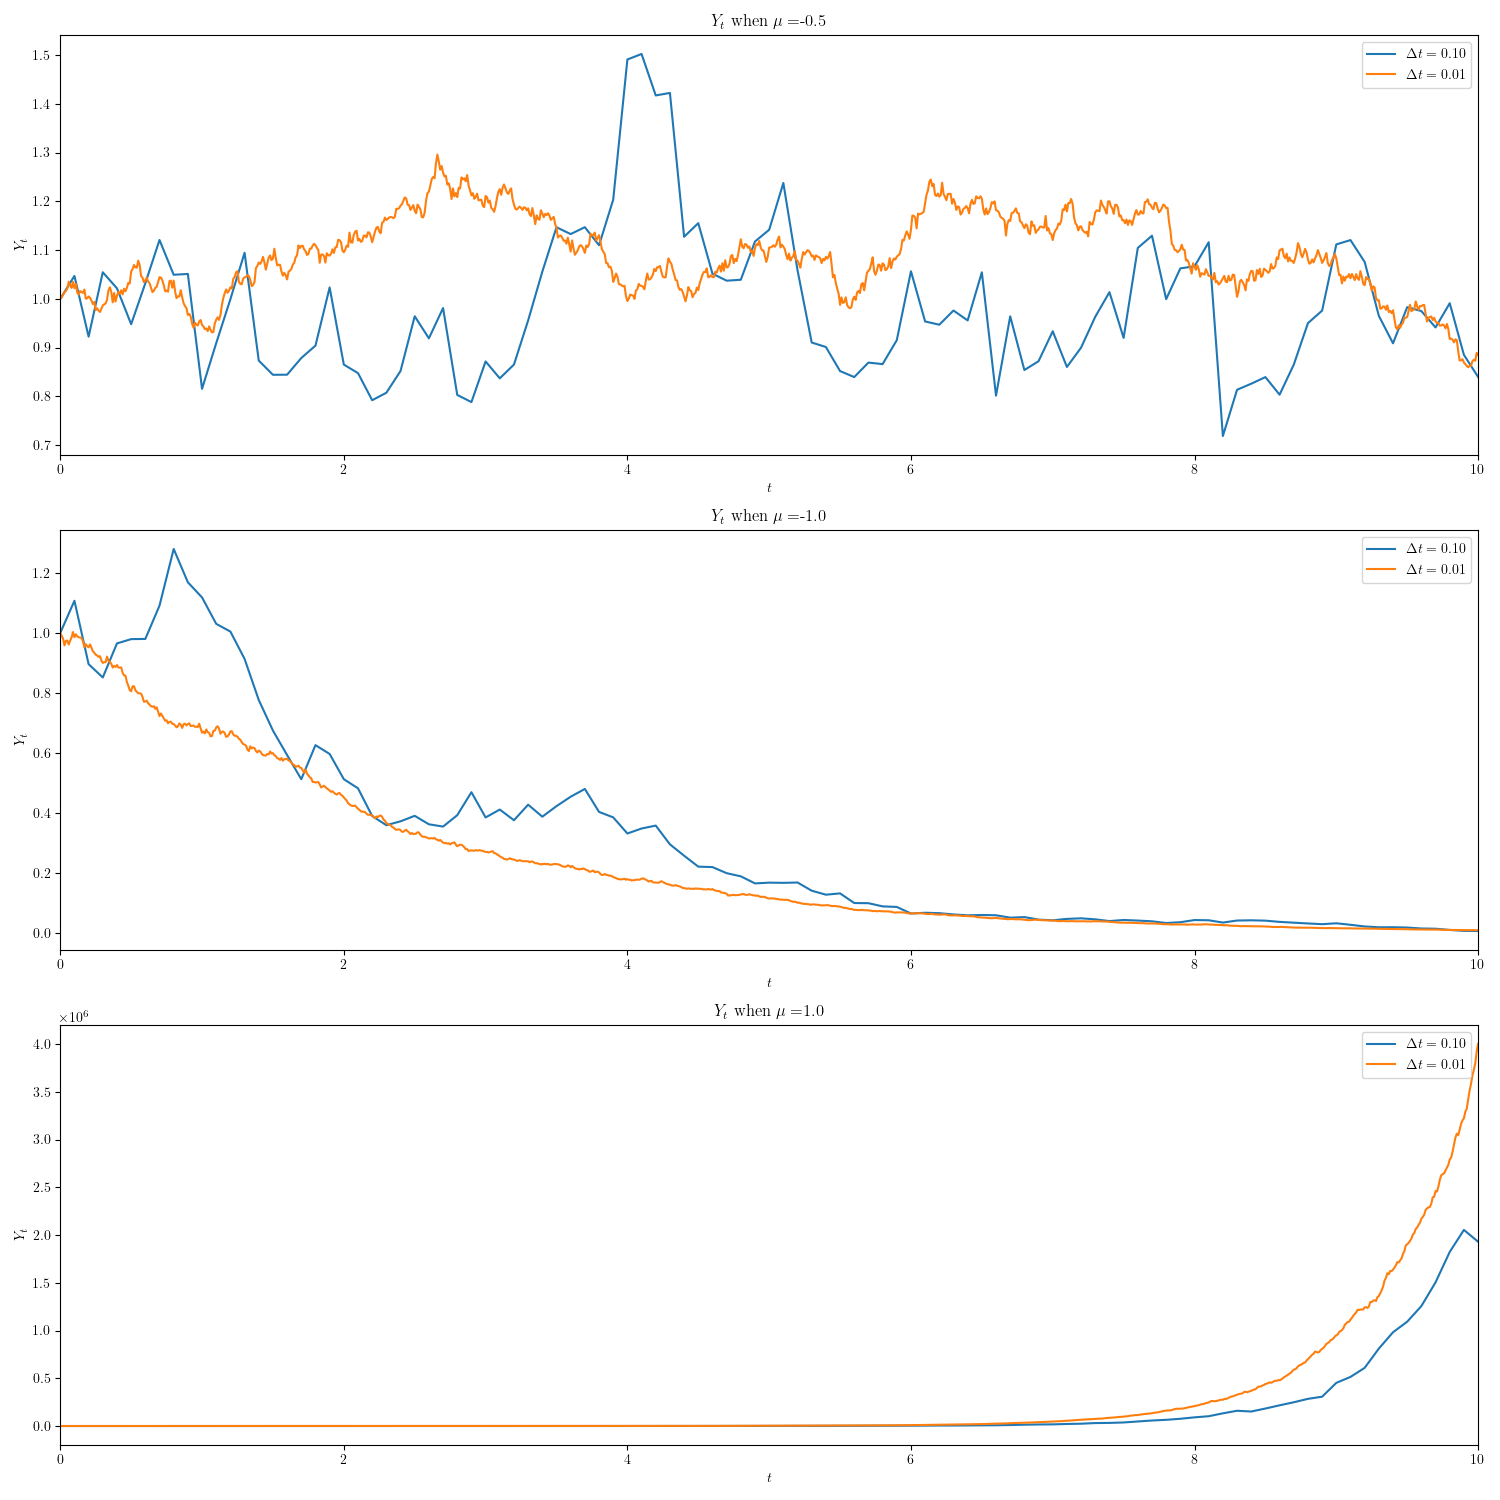
\includegraphics[width=18cm]{./Programming/Q3-1-D.png}
            \caption{Geometric Brownian Motion with $\mu = -1/2, \, -1 \; \& \; 1$ and $\Delta t = 0.1 \; \& \; 0.01$}
            \label{fig1}
        \end{figure}

\end{enumerate}
